\documentclass[11pt,letter]{amsart}
\usepackage[utf8]{inputenc}
\usepackage{graphicx}
\usepackage{amssymb}
\usepackage{amsmath}
\usepackage{epstopdf}
\usepackage{amsthm}
\usepackage{xypic}
\usepackage{enumerate}
%\usepackage{sidenotes}

%\usepackage{fourier}
%\usepackage{a4wide}


\newtheorem{definition}{Definition} 
\newtheorem{proposition}[definition]{Proposition} 
\newtheorem{theorem}[definition]{Theorem} 
\newtheorem{lemma}[definition]{Lemma} 
\newtheorem{corollary}[definition]{Corollary}
\newtheorem{conjecture}[definition]{Conjecture}
\newtheorem{question}[definition]{Question}
\newtheorem{claim}[definition]{Claim}
\newtheorem{fact}[definition]{Fact}
\newtheorem{remark}[definition]{Remark}
\newtheorem{wedgelemma}[definition]{Wedge Lemma} 
\newtheorem{construction}[definition]{Construction}
\newtheorem{example}[definition]{Example}

\newcommand{\lo}{\preceq}
\newcommand{\rar}{\rightarrow}
\newcommand{\rAr}{\Rightarrow}
\newcommand{\lrAr}{\Leftrightarrow}
\newcommand{\RR}{\mathbb{R}}
\newcommand{\NN}{\mathbb{N}}
\newcommand{\QQ}{\mathbb{Q}}
\newcommand{\ZZ}{\mathbb{Z}}
\newcommand{\HHH}{\mathcal{H}}
\newcommand{\AAA}{\mathcal{A}}
\newcommand{\K}{\mathbf{K}}
\renewcommand{\L}{\mathbf{L}}
\newcommand{\U}{\mathbf{U}}
\newcommand{\V}{\mathbf{V}}
\newcommand{\X}{\mathbf{X}}
\newcommand{\Rat}{\operatorname{Rat}}
\newcommand{\ehr}{\operatorname{ehr}}
\newcommand{\dist}{\mathsf{dist}}
\newcommand{\sgn}{\mathrm{sgn}}
\newcommand{\sprod}[2]{\langle #1, #2 \rangle}
\newcommand{\mspan}{\operatorname{span}}
\renewcommand{\dim}{\mathsf{dim}\ }
\newcommand{\inter}{\mathsf{int}\ }
\newcommand{\median}{\mathrm{median}\ }
\DeclareMathOperator*{\argmin}{arg\,min}

\newcommand{\defn}[1]{\emph{#1}}
\newcommand{\norm}[1]{|| #1 ||}

\newcommand{\Glat}{G^{\operatorname{lat}}}
\newcommand{\Gdep}{G^{\operatorname{dep}}}
\newcommand{\Gfine}{G^{\operatorname{fine}}}
\newcommand{\Gfinem}{G^{\operatorname{fine*}}}

\newcommand{\FD}{\mathcal{F}}
\newcommand{\path}{\operatorname{path}}
\newcommand{\reldep}[2]{{#1} \longrightarrow {#2}}
\newcommand{\reldepi}[3]{{#1} \overset{#2}{\longrightarrow} {#3}}
\newcommand{\shift}[2]{\rightarrow(#1,{#2})}
\newcommand{\shiftw}[3]{\overset{#1 \cdot #2}{\longrightarrow} {#3}}

\newcommand{\conv}{\operatorname{conv}}
\newcommand{\cone}{\operatorname{cone}}
\newcommand{\lev}{\operatorname{lev}}
\newcommand{\Lev}{\operatorname{Lev}}
\renewcommand{\deg}{\operatorname{deg}}
\renewcommand{\dim}{\operatorname{dim}}
\renewcommand{\min}{\operatorname{min}}
\renewcommand{\max}{\operatorname{max}}
\newcommand{\fract}{\operatorname{frac}}
\newcommand{\integ}{\operatorname{int}}
\newcommand{\relint}{\operatorname{relint}}

\newcommand{\twin}{\mathsf{twin}}
\newcommand{\hull}{\mathsf{hull}}
\newcommand{\diam}{\mathsf{diam}}
\newcommand{\choice}[1]{\left\{ \begin{array}{ll} #1 \end{array} \right.}
\newcommand{\floor}[1]{\lfloor {#1} \rfloor}
\newcommand{\ceil}[1]{\lceil {#1} \rceil}
\newcommand{\mset}[2]{ \left\{ #1 \; \middle| \; #2 \right\}}
\newcommand{\lk}{\mathsf{lk}}
\newcommand{\sd}{\mathsf{sd}}
\newcommand{\Pa}{\mathrm{P}}
\newcommand{\dotcup}{\ensuremath{\mathaccent\cdot\cup}}
\newcommand{\Hom}{\mathrm{ Hom}}


\title{Notes}
\author{Felix Breuer, Caroline J. Klivans}
\begin{document}
\maketitle


%%%%%%%%%%%%%%%%%%%%%%%%%%%%%%%%%
\section{Outline}
%%%%%%%%%%%%%%%%%%%%%%%%%%%%%%%%%

\begin{enumerate}
\item Flows and Hyperplane Arrangement Duality
\item Hopf Structure on Zonotopes/Hyperplane Arrangements in General
\item Scheduling Problems, Quasisymmetric Functions and Polynomials
\end{enumerate}


\noindent A motivating diagram:
\begin{equation*} \label{big_picture}
\xymatrix{
\textrm{colorings}  \dto &\textrm{Flows}\\
 \textrm{$\mathbb{Z}$ points in interiors of $G$-Braid} \dto & \textrm{$\mathbb{Z}$-points in interior} \uto\\
 \textrm{$G$-Braid} + \textrm{Coord.} \rto^{Duality}  & \textrm{$G$-subset arrangement} \uto}
\end{equation*}



%%%%%%%%%%%%%%%%%%%%%%%%%%%%%%%%%
\section{Hyperplane Arrangement Duality}
%%%%%%%%%%%%%%%%%%%%%%%%%%%%%%%%%

Let $V\subset \ZZ^d\setminus\{0\}$ be a finite set of primitive integer vectors.\footnote{Primitive means that the $\gcd$ of the entries of each vector is 1.} Let $\HHH$ denote the central hyperplane arrangement
\[
\HHH = \mset{H_v}{v\in V}
\]
where
\[
H_v = \mset{x\in \RR^d}{\sprod{x}{v}=0}.
\]
The cones in $\HHH$ are rational, whence their generators can be chosen to be primitive and integral. Let $G(V)$ denote the set of primitive integral generators of $\HHH$. In other words, $G(V)$ can be described as follows:
\[
 G(V) = \mset{w\in\ZZ^d\setminus\{0\}\text{ primitive}}{\exists T\subset V: \dim T^\perp = 1 \wedge w\in T^\perp}
\]
where $T^\perp = \mset{x\in\RR^d}{\sprod{x}{y}=0 \text{ for all} y\in T}$.

Note: Defined this way, $G(V)$ always produces a centrally symmetric set of vectors. We may or may not want this convention.

\begin{lemma}
$G$ maps a finite set of primitive lattice points to a finite set of primitive lattice points.
\end{lemma}

\begin{proof}
There are only finitely many subsets $T$ to choose from. If $\dim T^\perp = 1$ and $T$ is rational there are exactly two primitive non-zero lattice points in  $T^\perp$.
\end{proof}

\begin{lemma}
Let $V,W\subset \ZZ^d\setminus\{0\}$ be a finite sets of primitive integer vectors that span $\RR^d$. Then 
\begin{enumerate}
\item $V\subset W$ $\rAr$ $G(V)\subset G(W)$,
\item $V \subset G(G(V))$.
\end{enumerate}
\end{lemma}

\begin{proof}
(1) If $W\supset V$ then in the definition $G(W)$ there are more subsets $T$ to choose from than in the definition of $G(V)$.

(2) Let $v\in V$. Define $v_1:=v$ and let $v_2,\ldots,v_d\in V$ such that $v_1,v_2,\ldots,v_d$ is a basis for $\RR^d$. Let $V_i=\{v_1,\ldots,v_d\}\setminus\{v_i\}$. Then $\dim V_i^\perp = 1$ for every $i$. Moreover, if $w\in V_i^\perp$ for $i=2,\ldots,d$, then $w\perp v$. Let $w_i$ denote a primitive lattice vector in $V_i^\perp$. By construction $w_i\in G(V)$. Moreover, $w_2,\ldots,w_d$ are linearly independent\footnote{What's a good proof for linear independence of the $w_i$?}, so $\dim \{w_2,\ldots,w_d\}^\perp=1$ and $v\in \{w_2,\ldots,w_d\}^\perp$, whence $v\in G(G(V))$ as desired.  
\end{proof}


\subsection{Hyperplane arrangements}

I simply want to talk through the above in a different way.  

Suppose $\mathcal{H}$ is a finite central hyperplane arrangement and $V$ is
the collection of all normals to the hyperplanes $H \in \mathcal{H}$.
Suppose further that $V$ is a collection of primitive integer vectors.

\begin{quote}
C: I actually don't know what this means for $\mathcal{H}$.  Namely,
which arrangements have primitive integer normals?  If I describe an
arrangement in terms of linear forms with integer coefficients, then
do I just need a gcd condition on those coefficients?

F: Yes! We just need that $\gcd(v_1,v_2,\ldots,v_d)=1$ for every normal $v$. So all we really need is a rational hyperplane arrangement.
\end{quote}

Next we consider the collection of generators of all cones of
$\mathcal{H}$.  As $\mathcal{H}$ is determined by $V$, we may write
this as a function of $V$, $G(V)$.  

\begin{quote}
C: I think you need to be careful in your definition of $G(V)$ above.
If the arrangement is not essential, then we will not see all the
generators of cones as one dimensional intersections.  Consider the
Braid arrangement as it sits in $\mathbb{R}^3$.  This arrangement is
not essential and the cones only have one one-dimensional face - the
common intersection of all hyperplanes.  Do we want to work with an
essentialization?

F: Good point! I can't think of a way to get arround the assumption that the arrangement is essential. Do we know that if $V$ is essential, then $G(V)$ is essential as well?
\end{quote}

Now $G(V)$ is a collection of primitive integer vectors (Lemma 1).  We
can interpret $G(V)$ as a collection of normals of a new hyperplane
arrangement $\mathcal{H}^*$.

Lemma 2 shows that:
\begin{enumerate}
\item If $\mathcal{H} \subseteq \mathcal{K}$ then $\mathcal{H}^* \subseteq \mathcal{K}^*$.
\item $\mathcal{H} \subseteq (\mathcal{H}^*)^*$.
\end{enumerate}

\begin{question}
When is the dual of the dual the original arrangement?  $\mathcal{H} =
(\mathcal{H}^*)^*$ ?  The second part of the Lemma says that we get
back at least $\mathcal{H}$ but we might pick up more.  Can we give a
nice describe of the extra hperplanes we pick up?  Can we describe the
dual of the dual directly from the intersection lattice?
\end{question}

\begin{example}

We should write out the example with $\mathcal{H} = $ Braid arrangement
plus coordinate hyperplanes in $\mathbb{R}^3$.  The dual is then the
all subsets arrangement.  The dual of the dual is not the original.

\end{example}

\begin{figure}
\includegraphics[width=12cm]{duality}
\caption{Dual of braid arrangement. Could use a less messy picture.}
\end{figure}

We can give an explicit formula for the vectors appearing in the dual arrangement. Given $d$ linearly independent vectors $v_1,\ldots,v_{d}$ in $\RR^d$, the $1$-dimensional linear space given by
\[
  \sprod{v_1}{x} = \sprod{v_2}{x} = \ldots = \sprod{v_{d-1}}{x} = 0
\]
is spanned by the unique solution to the linear system $Ax=e_d$ where $A$ is the matrix with \emph{rows} $v_1,\ldots,v_d$. That is, if we have $d$ linearly independent normal vectors $v_1,\ldots,v_d$ from our arrangement, then $d$ vectors in the dual are given by
\[
  \operatorname{prim}(A^{-1} e_i) \text{ for } i=1,\ldots,d
\]
where $\operatorname{prim}(x)$ is the unique primitive integer vector that is a  positive multiple of $x$.\footnote{In other words, $\operatorname{prim}(x)$ is the integral multiple $\lambda x$ for which $\lambda> 0$ is minimal.} Using Cramer's rule, we can obtain a formula for the vectors $A^{-1}e_i$, namely
\[
  A^{-1}e_i = \frac{1}{\det A}\sum_{j=1}^d \det(w_1,\ldots,w_{i-1},e_i,w_{i+1},\ldots, w_d)\cdot e_j,
\]
where the $w_i$ are the \emph{columns} of $A$.

This is certainly reminiscent of the formula given in the Bayer--Brandt article for the discriminantal arrangement. But it is not the same, simply for the fact that the discriminantal arrangement takes $n$ vectors in $\RR^k$ and produces an arrangement in $\RR^n$ with $n>k$.

Nonetheless, this allows us to give an explicit formula for computing the dual.

\begin{lemma}
Let $V$ be a finite set of primitive integral vectors in $\RR^d$ such that if $v\in V$ then $-v\in V$ and $V$ contains a subset of at least $d$ linearly independent vectors.\footnote{This last part guarantees that the arrangement is essential.} Then $G(V)$ is given by
\[
  G(V) = \mset{\operatorname{prim}(\pm A_S e_d)}{ S\subset V, |S|=d-1, \text{$S$ linearly independent} },
\]
where $A_S$ denote the square matrix that has the vectors in $S$ as rows and one more row that is linearly independent of the others but otherwise chosen arbitrarily.
\end{lemma}

\begin{quote}
F: I will implement this in Sage and see what happens.
\end{quote}



\section{Hopf Monoids}

Define Hopf monoid?  

In previous work [ABK], given a Hopf monoid and a character map, one
associates a pair of related objects, an element of NCQsym
(quasisymmetric function in non-commuting variables) and a simplicial
complex.  

Especially nice things can be said when one works with generalized
permutahedron.  Aguair and Ardila defined a Hopf monoid of generalized
permutahedron and investigated the behavior of the following choice of
character map:

\begin{displaymath}
\zeta(P) = \left\{ \begin{array}{ll}
1 & \textrm{ if $P$ is a point}, \\
0 & \textrm{ otherwise}
\end{array} \right.
\end{displaymath}


Generalized permutahedron include graphical zonotopes and matroid
polytopes.  In the case of graphical zonotopes, the quasisymmetric
function in non-commuting variables mentioned above is the ``chromatic
NCQsym'' of the graph.  It specializes to Stanley's chromatic
(quasi)-symmetric function and hence to the chromatic polynomial of a
graph.

(Explain how all this works and that all you are really doing is
taking the lattice points in the interior of the normal fan of the
graphical zonotope.)

\subsection{Zonotopes}

In it's most general form, the construction above works for any Hopf
monoid and character map.  On the other hand, quasisymmetric functions
and even more obviously NCQsym elements naturally live in the same
picture as generalized permutahedron.  (Because these are exactly the
polytopes whose normal fans are refined by the Braid arrangement).

We have reason to work with polytopes / arrangements that are not GPs
/ Braid.  Can we construct a Hopf monoid structure for
zonotopes?  

\subsection{Hopf Monoid of Hyperplane Arrangements?}

I have been brainstorming with Jeremy on how one might define a Hopf monoid of hyperplane arrangements. Here are some ideas that try to generalize what is happening in the Hopf monoid of graphs when viewed through the lens of the graphic arrangement. 

For any set $S\subset[n]$ of indices, we let $A(S)$ denote the corresponding coordinate subspace in $\RR^n$, i.e.,
\[
  A(S) = \{ x\in\RR^n | x_i=0 \;\;\forall i\in S\}.
\]
Given a hyperplane arrangement $\HHH$ and a coordinate subspace $A$, we define the hyperplane arrangement $\HHH_A$ projected onto the orthogonal complement of $A$ by
\[
  \HHH_A = \{ H/A \; | \;  H\in\HHH \text{ and } A\subset H\}.
\]
That is we keep only those hyperplanes that contain $A$ and then quotient out $A$. For example, let $\HHH$ be the Braid arrangement in $\RR^3$ and let $A=\{x| x_1=x_2=0\}$. Then $\HHH_A$ is the arrangement in $\RR^2$, i.e. "$x_1$-$x_2$-space", consisting of the single hyperplane $\{x|x_1=x_2\}$. The projection of the hyperplane $\{x|x_1=x_3\}$ is not contained in $\HHH_A$ because it does not contain $A$.

\begin{figure}
\includegraphics[width=6cm]{monoid}
\caption{Example projection $\HHH_A$.}
\end{figure}


We can use this to define a coproduct $\Delta$ by
\[
\Delta\HHH = \sum_{S\subset[n]} \HHH_{A(S)} \otimes \HHH_{A(S^c)}
\]
where $\HHH$ is a hyperplane arrangement in $\RR^n$ and $S^c$ denotes the complement of $S$ in $[n]$.

The corresponding product would be
\[
  \HHH_1 \cdot \HHH_2 = \{H \oplus \RR^m | H\in \HHH_1 \} \cup \{R^n \oplus H | H\in \HHH_2 \}
\]
where $\HHH_1$ is an arrangement in $\RR^n$ and $\HHH_2$ is an arrangement in $\RR^m$.

This seems to give a Hopf monoid/Hopf algebra. However, the algebraic structure depends only on the supports of the normal vectors. So rather than producing an inherently geometric Hopf algebra this seems to give rather a Hopf algebra of hypergraphs.


%%%%%%%%%%%%%%%%%%%%%%%%%%%%%%%%%
\section{Scheduling Problems}
%%%%%%%%%%%%%%%%%%%%%%%%%%%%%%%%%

A \defn{scheduling problem} $S$ on $d$ items is given by a boolean formula $\phi$ over atomic formulas $x_i\leq x_j$ for $i,j\in[d]$. A \defn{$k$-schedule} solving $S$ is a function $x:[d]\rightarrow[k]$ such that $\phi(x)$ is true. The schedule function $\xi_S(k)$ counts the number of $k$-schedules of $S$.

From the standard braid arrangement setup, we get the following results:
\begin{enumerate}
\item $\xi_S(k)$ is a polynomial in $k$.
\item There is a natural quasisymmetric function in non-commuting variables that specializes to $\xi_S$.
\item $\xi_S$ includes the chromatic polynomial of a graph and the "unknown" matroid polynomial as special cases.
\item $\xi_S$ includes Ehrhart polynomials of order polytopes as a special case.
\item The values of $\xi_S(-k)$ at negative integers can be written as a difference of two counting functions. (This gives "one half" of a reciprocity theorem.) This should also be true on the quasisymmetric function level.
\item We get some elementary bounds on the coefficients of $\xi_S$. For example, the $f^*$-vector is non-negative. 
\end{enumerate}

This is of course just the start. We call schedules $S$ \defn{nice} that give rise to a unit cube with a co-dimension 1 subcomplex removed, such that the regions are open full-dim polytopes. Then:
\begin{enumerate}
\item If $S$ is nice, we get an honest reciprocity theorem, both on the quasisymmetric function level as well as on the polynomial level.
\item This case still includes chromatic polynomials and the matroid polynomials.
\item We get strong bounds on the coefficients of the polynomial in the Ehrhart setting (coming from convex ear decompositions).
\end{enumerate}

Of course there are still a bunch of things that are not clear at all, yet:
\begin{enumerate} 
\item Do the convex ear decompositions also tell us something about coefficients on the quasisymmetric function level?
\item Which schedules come from matroids? 
\end{enumerate}



\subsection{Motivating examples}

Given a graph, most naturally we consider the graphical arrangement,
the subarrangement of the Braid arrangement given by hyperplanes
indexed by edges in the graph.

Given a matroid, we consider the matroid polytope formed by the convex
hull of the support vectors of bases.  The normal fan of the matroid
polytope is refined by the Braid arrangement, but this fan and the
graphical arrangement are not the same.  

We considered the very special case of graphical matroids.  Matroids
whose bases correspond to spanning trees of a graph.  Take the
\emph{matroid polytope} approach to a graphical matroid.  What integer
points / weight classes / relative orderings are induced?  We saw more
complicated 'rules', for example:\\

$x_1 \neq x_2$ if $x_3 \geq x_1$.  But $x_1 = x_2$ is ok if $x_3 < x_1$.\\

We interpreted this as {\bf{scheduling}} of tasks.  Tasks $x_1$ and
$x_2$ can be performed  at the same time only if $x_3$ happens first.

\begin{figure}
\includegraphics[width=13cm]{graph-matroid}
\caption{Difference between graph construction and graphical matroid construction.}
\end{figure}


\begin{figure}
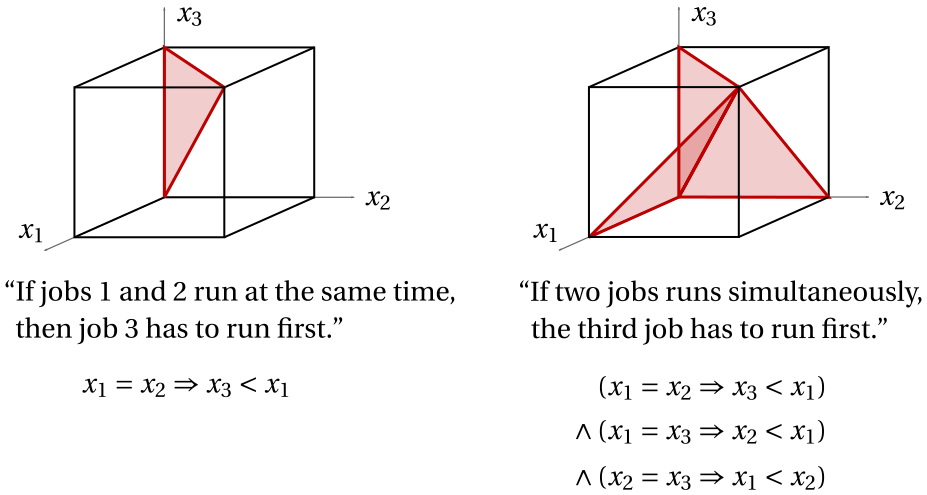
\includegraphics[width=13cm]{schedule}
\caption{Two "scheduling arrangements".}
\end{figure}



\bibliographystyle{amsplain}
\bibliography{references}

\end{document}
